\section{Systemarkitektur}
\subsection{Udkast fra Lund}
I dette afsnit vil systemarkitekturen for projektet blive beskrevet. Systemarkitekturen tager udgangspunkt i dokumentationsdokumentet "Systemarkitektur", og for nærmere uddybning henvises der til det dokument. 
Systemarkitekturen er udarbejdet på grundlag af kravspecifikationen og systemet som beskrevet i projektbeskrivelsen.

Systemarkitekturen starter med funktionaliteten beskrevet i Use Casene, og udvider så beskrivelsen til, at omfatte de elementer af systemet som brugeren ikke interagerer med. Dette afsnit vil give et eksempel på, hvordan en Use Case er blevet behandlet i systemarkitekturen. Use Casen der vil blive brugt som eksempel vil være Use Case 2: Skibsfører slår automatisk hældningsregulering til.

\begin{figure}[H]
\centering
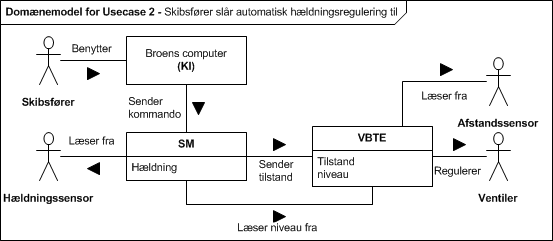
\includegraphics[scale=0.8]{billeder/Systemarkitektur/DM_UC2}
\caption{Domænemodel for Use Case 2}
\label{fig:dmuc2}
\end{figure}

\begin{figure}[H]
\centering
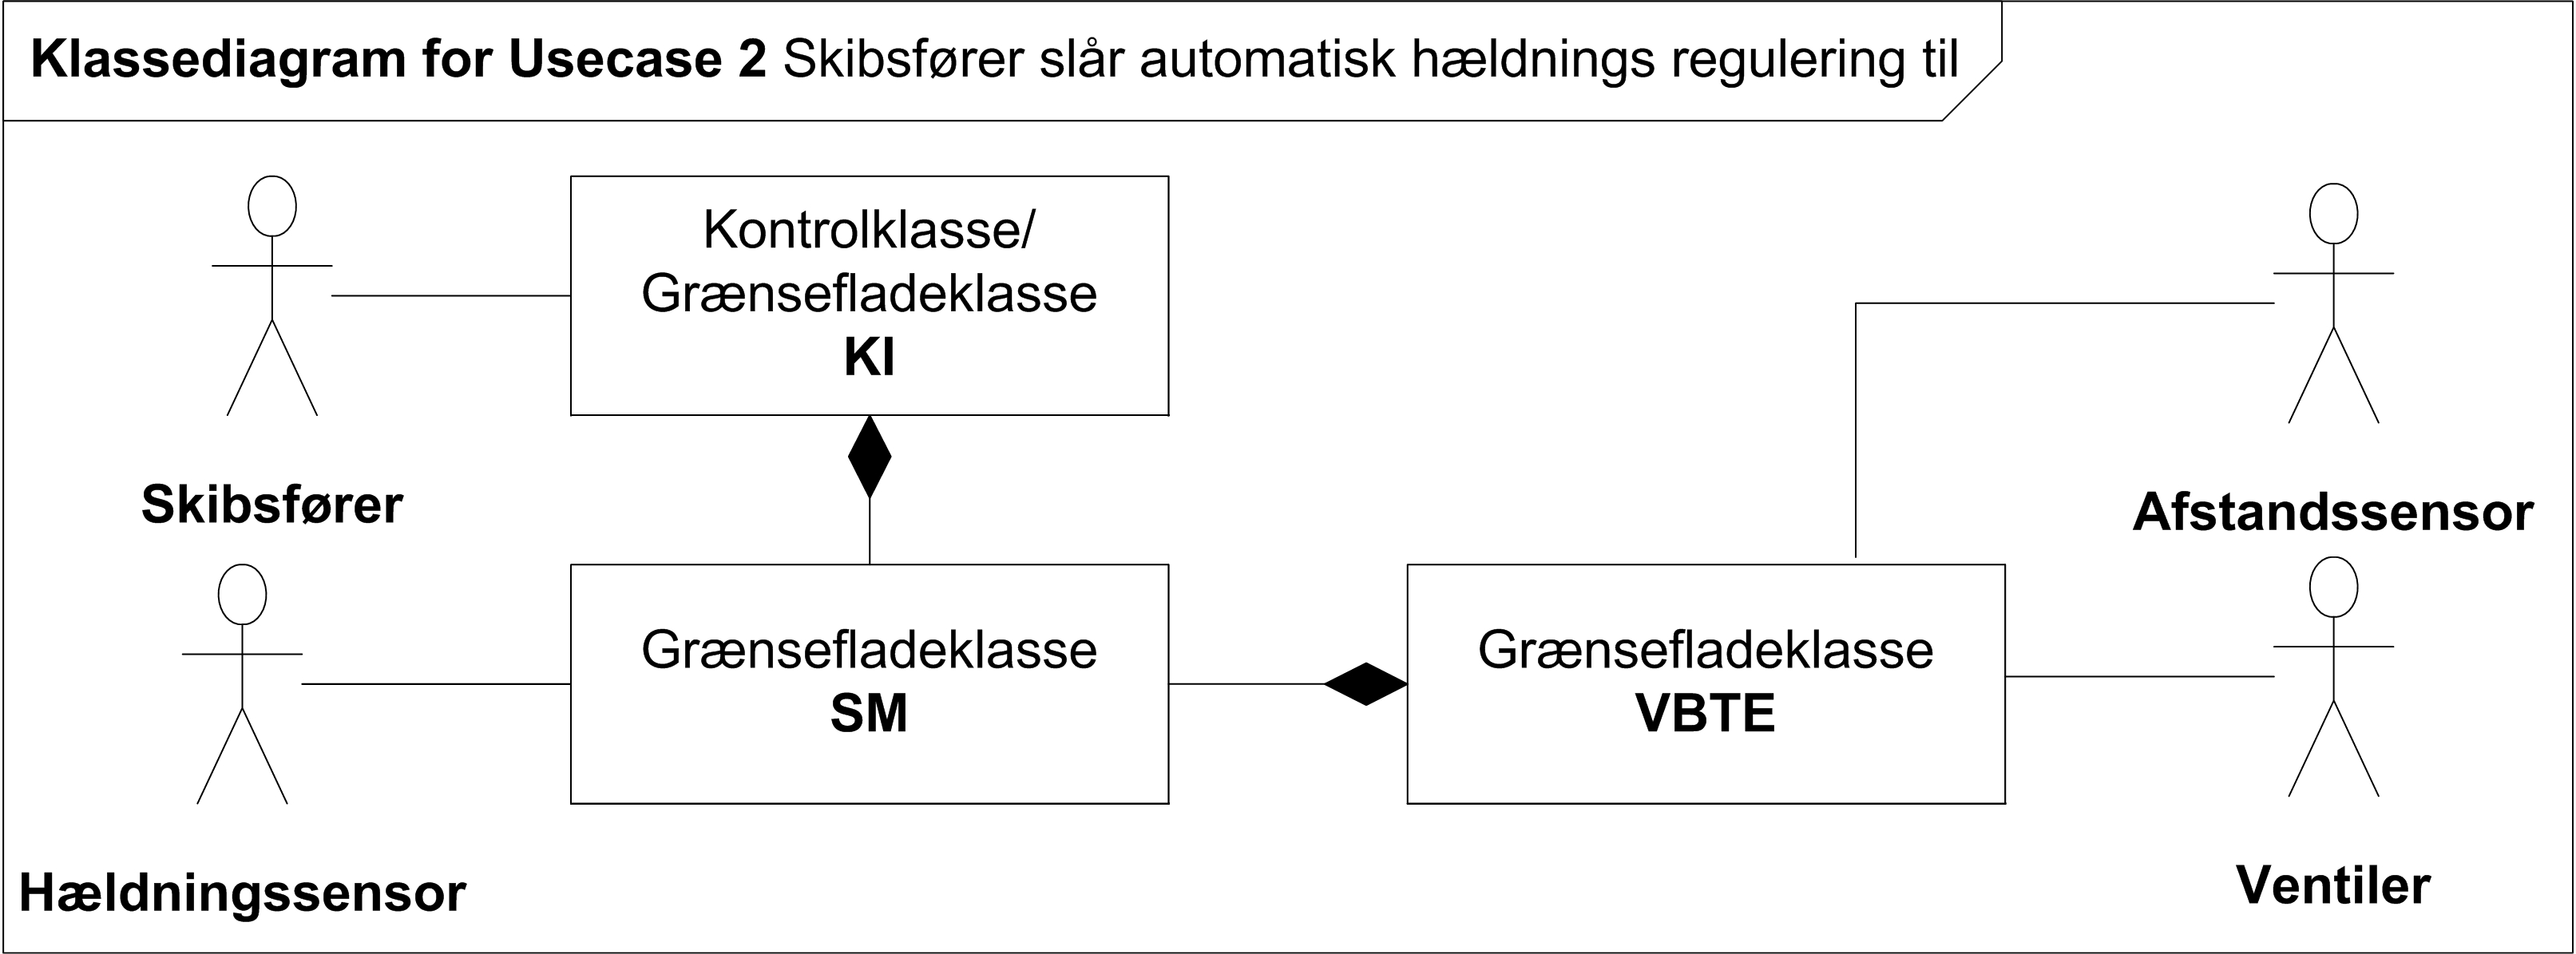
\includegraphics[scale=0.8]{billeder/Systemarkitektur/KD_UC2}
\caption{Klassediagram for Use Case 2}
\label{fig:kduc2}
\end{figure}

\begin{figure}[H]
\centering
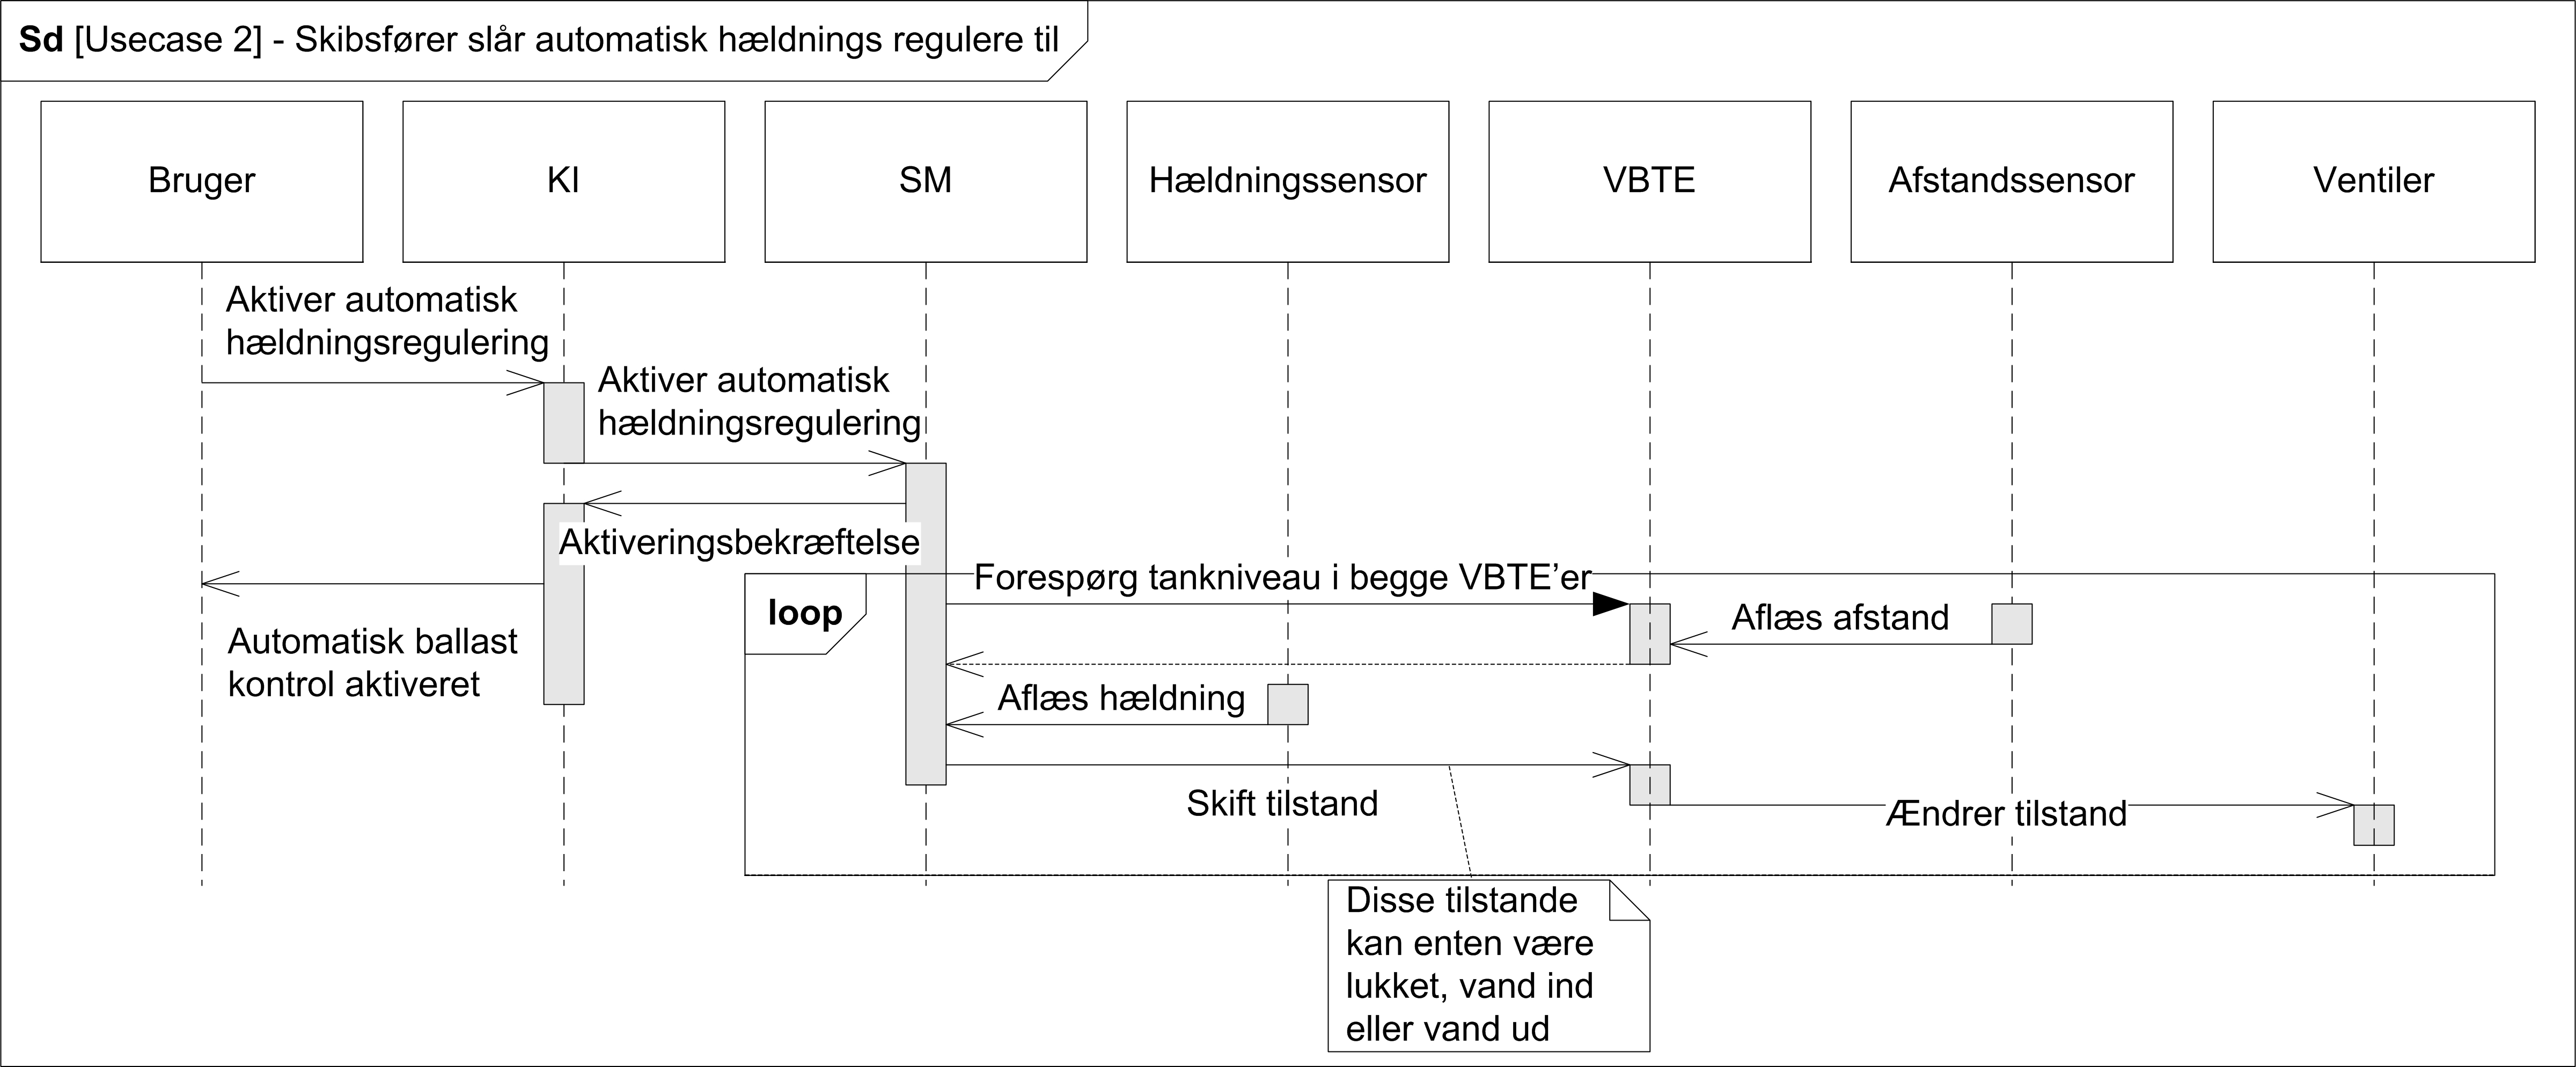
\includegraphics[scale=0.8]{billeder/Systemarkitektur/SD_UC2}
\caption{Sekvensdiagram for Use Case 2}
\label{fig:sduc2}
\end{figure}

I domænemodelen (figur \ref{fig:dmuc2}) beskrives relationen mellem systemets elementer og aktørerne. Disse enheder omdannes i klassediagrammet (figur \ref{fig:kduc2}) til konceptuelle klasser, af en given type. Det ses at i Use Case 2 agerer KI som både en kontrolklasse og en grænsefladeklasse. Den agerer som en kontrolklasse fordi den er initiativtager, og beslutningstager til den efterfølgende udvikling i systemet. Både KI, SM og VBTE agerer som en grænsefladeklasse, fordi alle tre klasser er i berøring med en aktør.\\
I sekvensdiagrammet (figur \ref{fig:sduc2}) beskrives kommunikationen og timingen imellem klasserne. Det ses at brugeren igangsætter processen, KI videresender kommandoen, SM bekræftiger modtagelsen af kommandoen, hvorefter den begynder at regulere på vandniveauet i tankene ved hjælp af VBTE'erne. Reguleringen sker på grundlag af de målinger den modtager fra hældningssensoreren. Vandniveauet vil blive ved med at blive reguleret, med et formål at opnå og derpå opretholde en hældning på nul grader.

\begin{figure}[htbp]
\centering
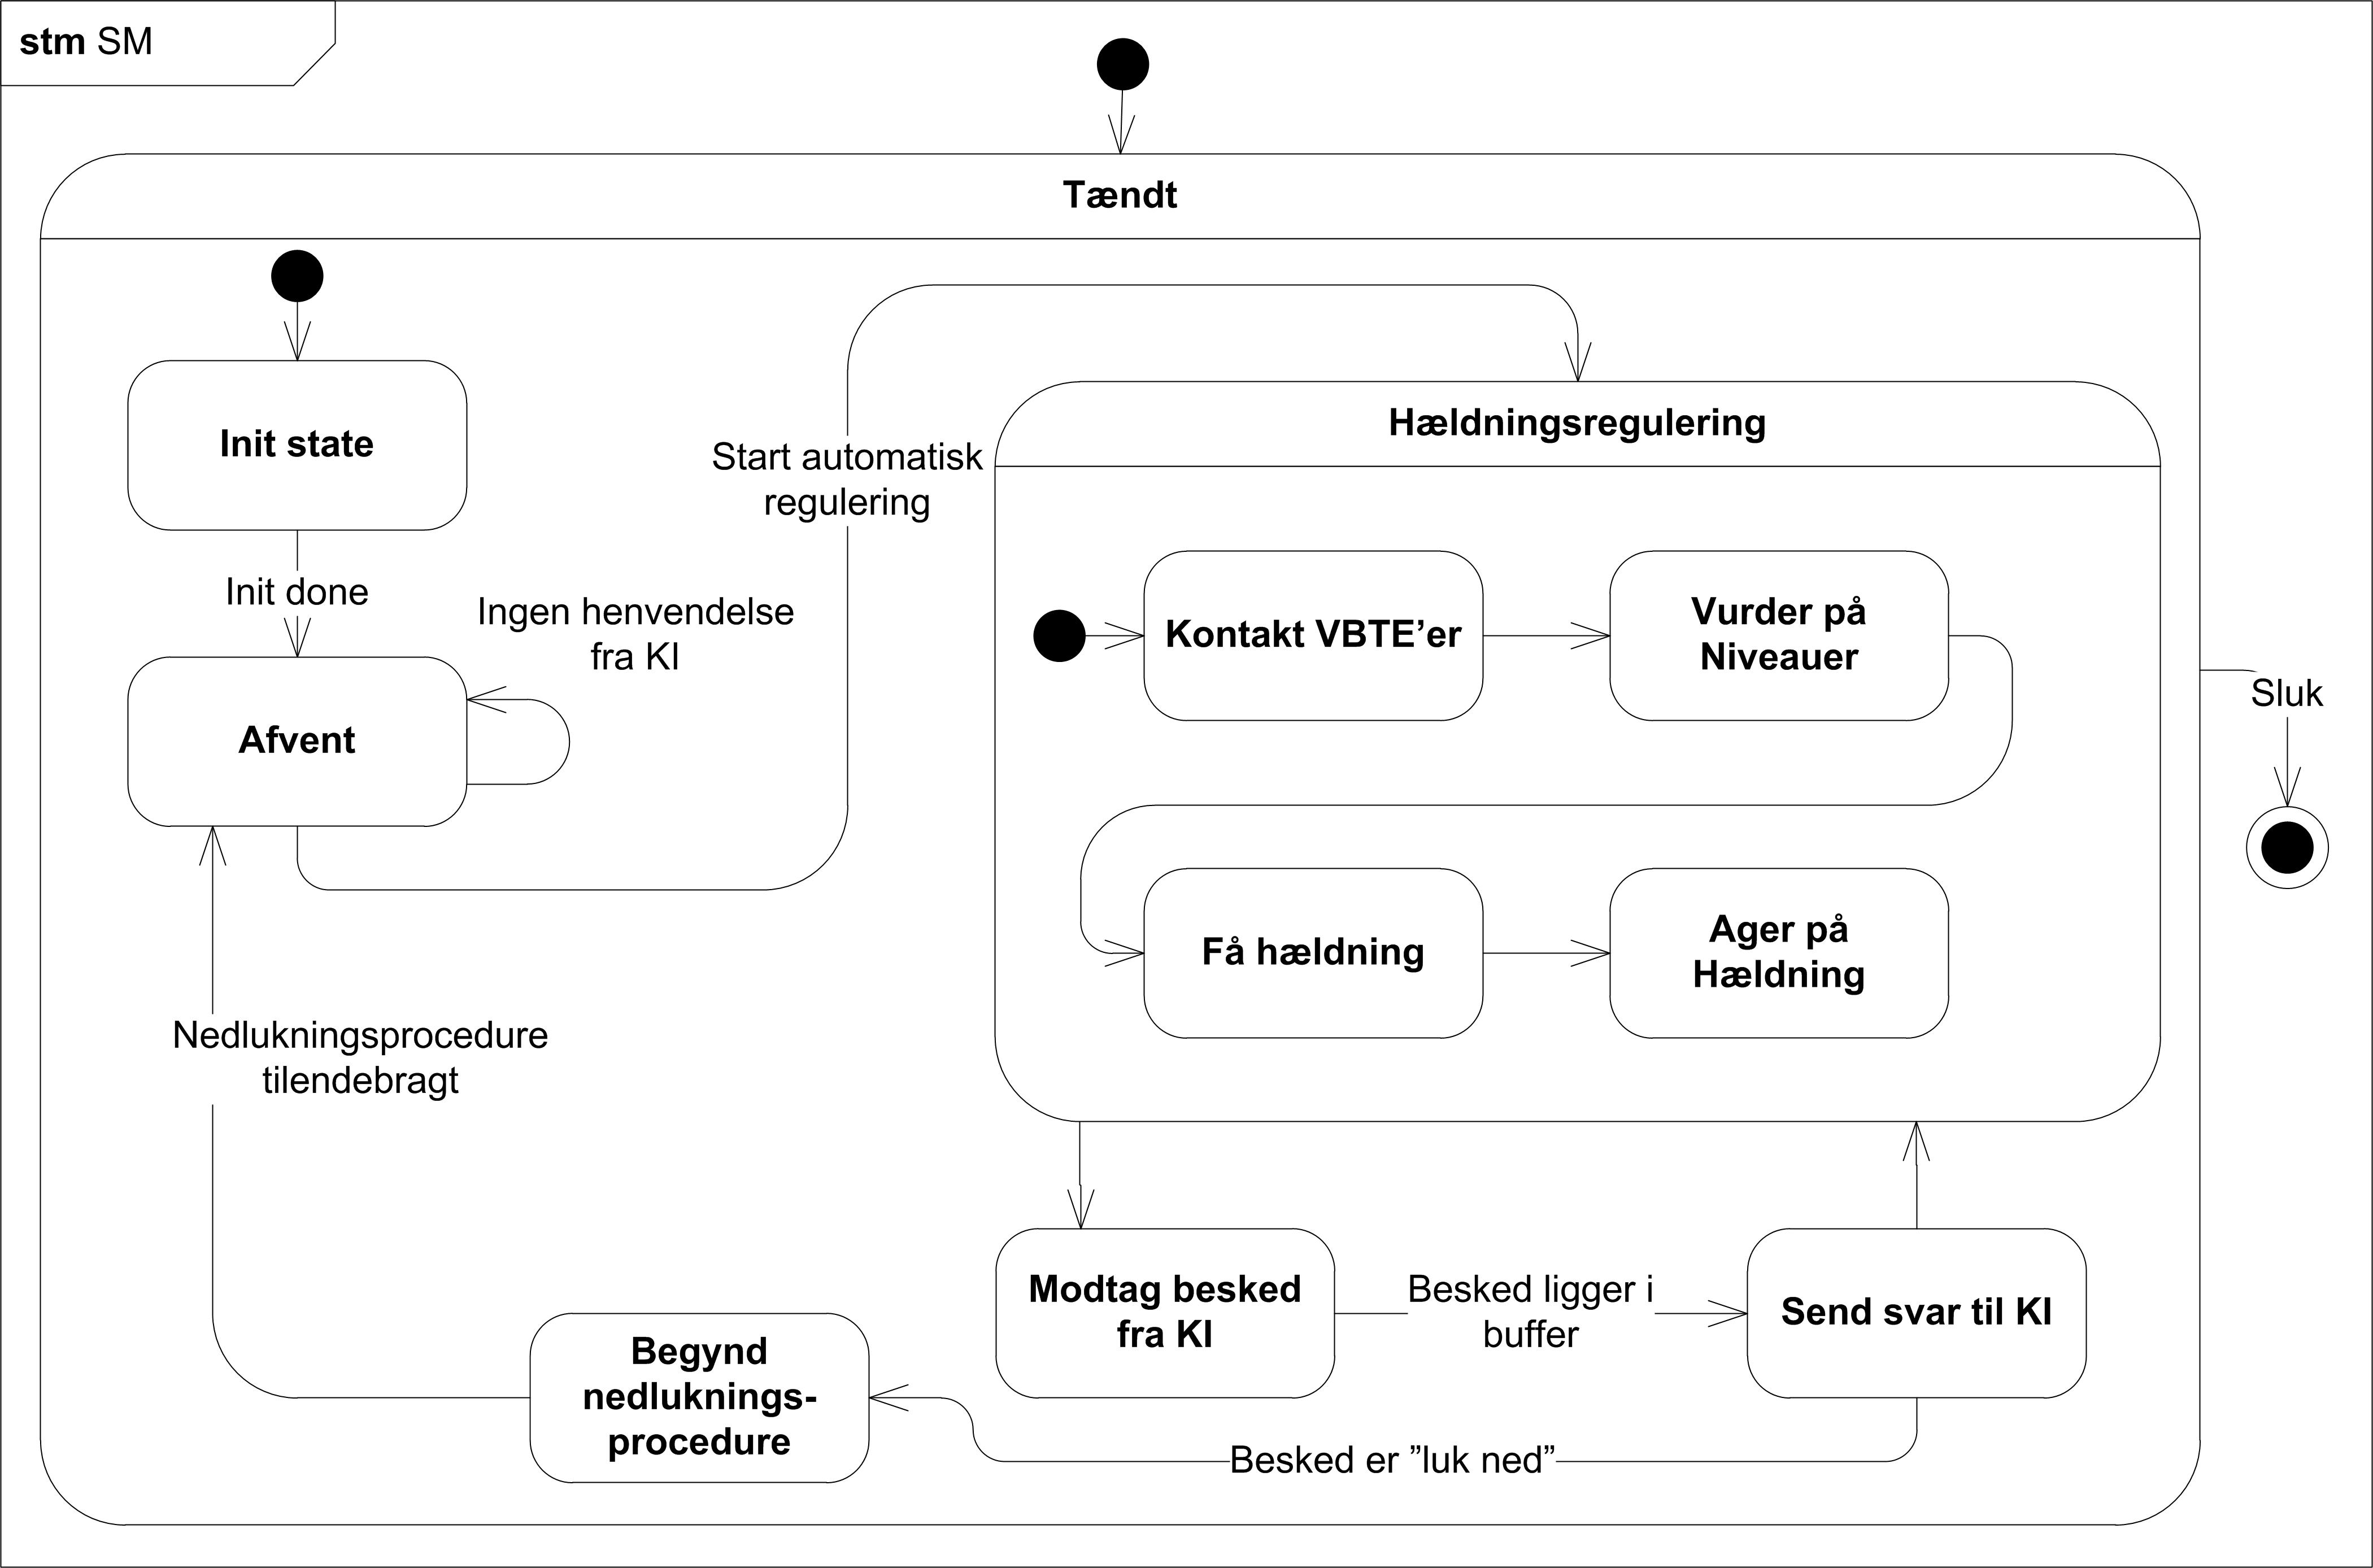
\includegraphics[scale=0.8]{billeder/Systemarkitektur/stm_sm}
\caption{State machine for Styringsmodulet}
\label{fig:stm_sm}
\end{figure}

Når alle Use Cases er blevet bearbejdet som Use Case 2 er blevet i figur \ref{fig:dmuc2}, \ref{fig:kduc2} og \ref{fig:sduc2} har gruppen dannet state machines for de konceptuelle klasser i systemet. Her visualiseres hvilke stadier, klasserne har brug for at gennemgå i løbet af klassens levetid, for at opfylde kravene sat i kravspecifikationen. Som et eksempel på en sådan state machine, vises state machinen for Styringsmodulet på figur \ref{fig:stm_sm}. \\Flowet i state machinen bygger oven på det beskrevne i sekvensdiagrammerne. Starten på Use Case 2, er et brugerinput på KI'en. Dette medfører en besked fra KI til SM. Programmet kan være i to forskellige stadier når den modtager beskeden:\\
Hvis programmet er nyopstartet, vil beskeden få styringsmodulet ud af "Afvent" -stadiet og til at aktivere automatisk hældningsregulering. Hvis programmet befinder sig i "Hældningsregulerings"-stadiet med reguleringstypen \textit{manuel}, vil beskeden fra KI få styringsmodulet over i stadiet "Modtaget besked fra KI". SM besvarer beskeden med en aktiveringsbekræftigelse, og programmet returerner derpå til "Hældningsregulering"-stadiet - nu med reguleringstypen \textit{automatisk}.

Dette var for Use Case 2. Der i state machinen beskrevet styringsmodulets opførelse i alle Use Case tilfælde. 

Næste trin er, at omdanne de konceptuelle klasser til et regulært system. Nogle konceptuelle klasser, kan grupperes, andre står for sig selv. Den fysiske opbygning af systemet, bliver så vist i et blokdefinitionsdiagram. Blokdefinitionsdiagrammet for 
systemet, kan ses i figur \ref{fig:bdd_bros}. Her ses det, at systemet ender ud med fire hovedblokke: Kontrolinterfacet, Styringsmodul, Vandballasttankenhed og Database. De konceptuelle klasser der ikke er endt som hovedblokke, er i stedet for blevet til underblokke af enten styringsmodulblokken eller vandballasttankenhedblokken.

\begin{figure}[htbp]
\centering
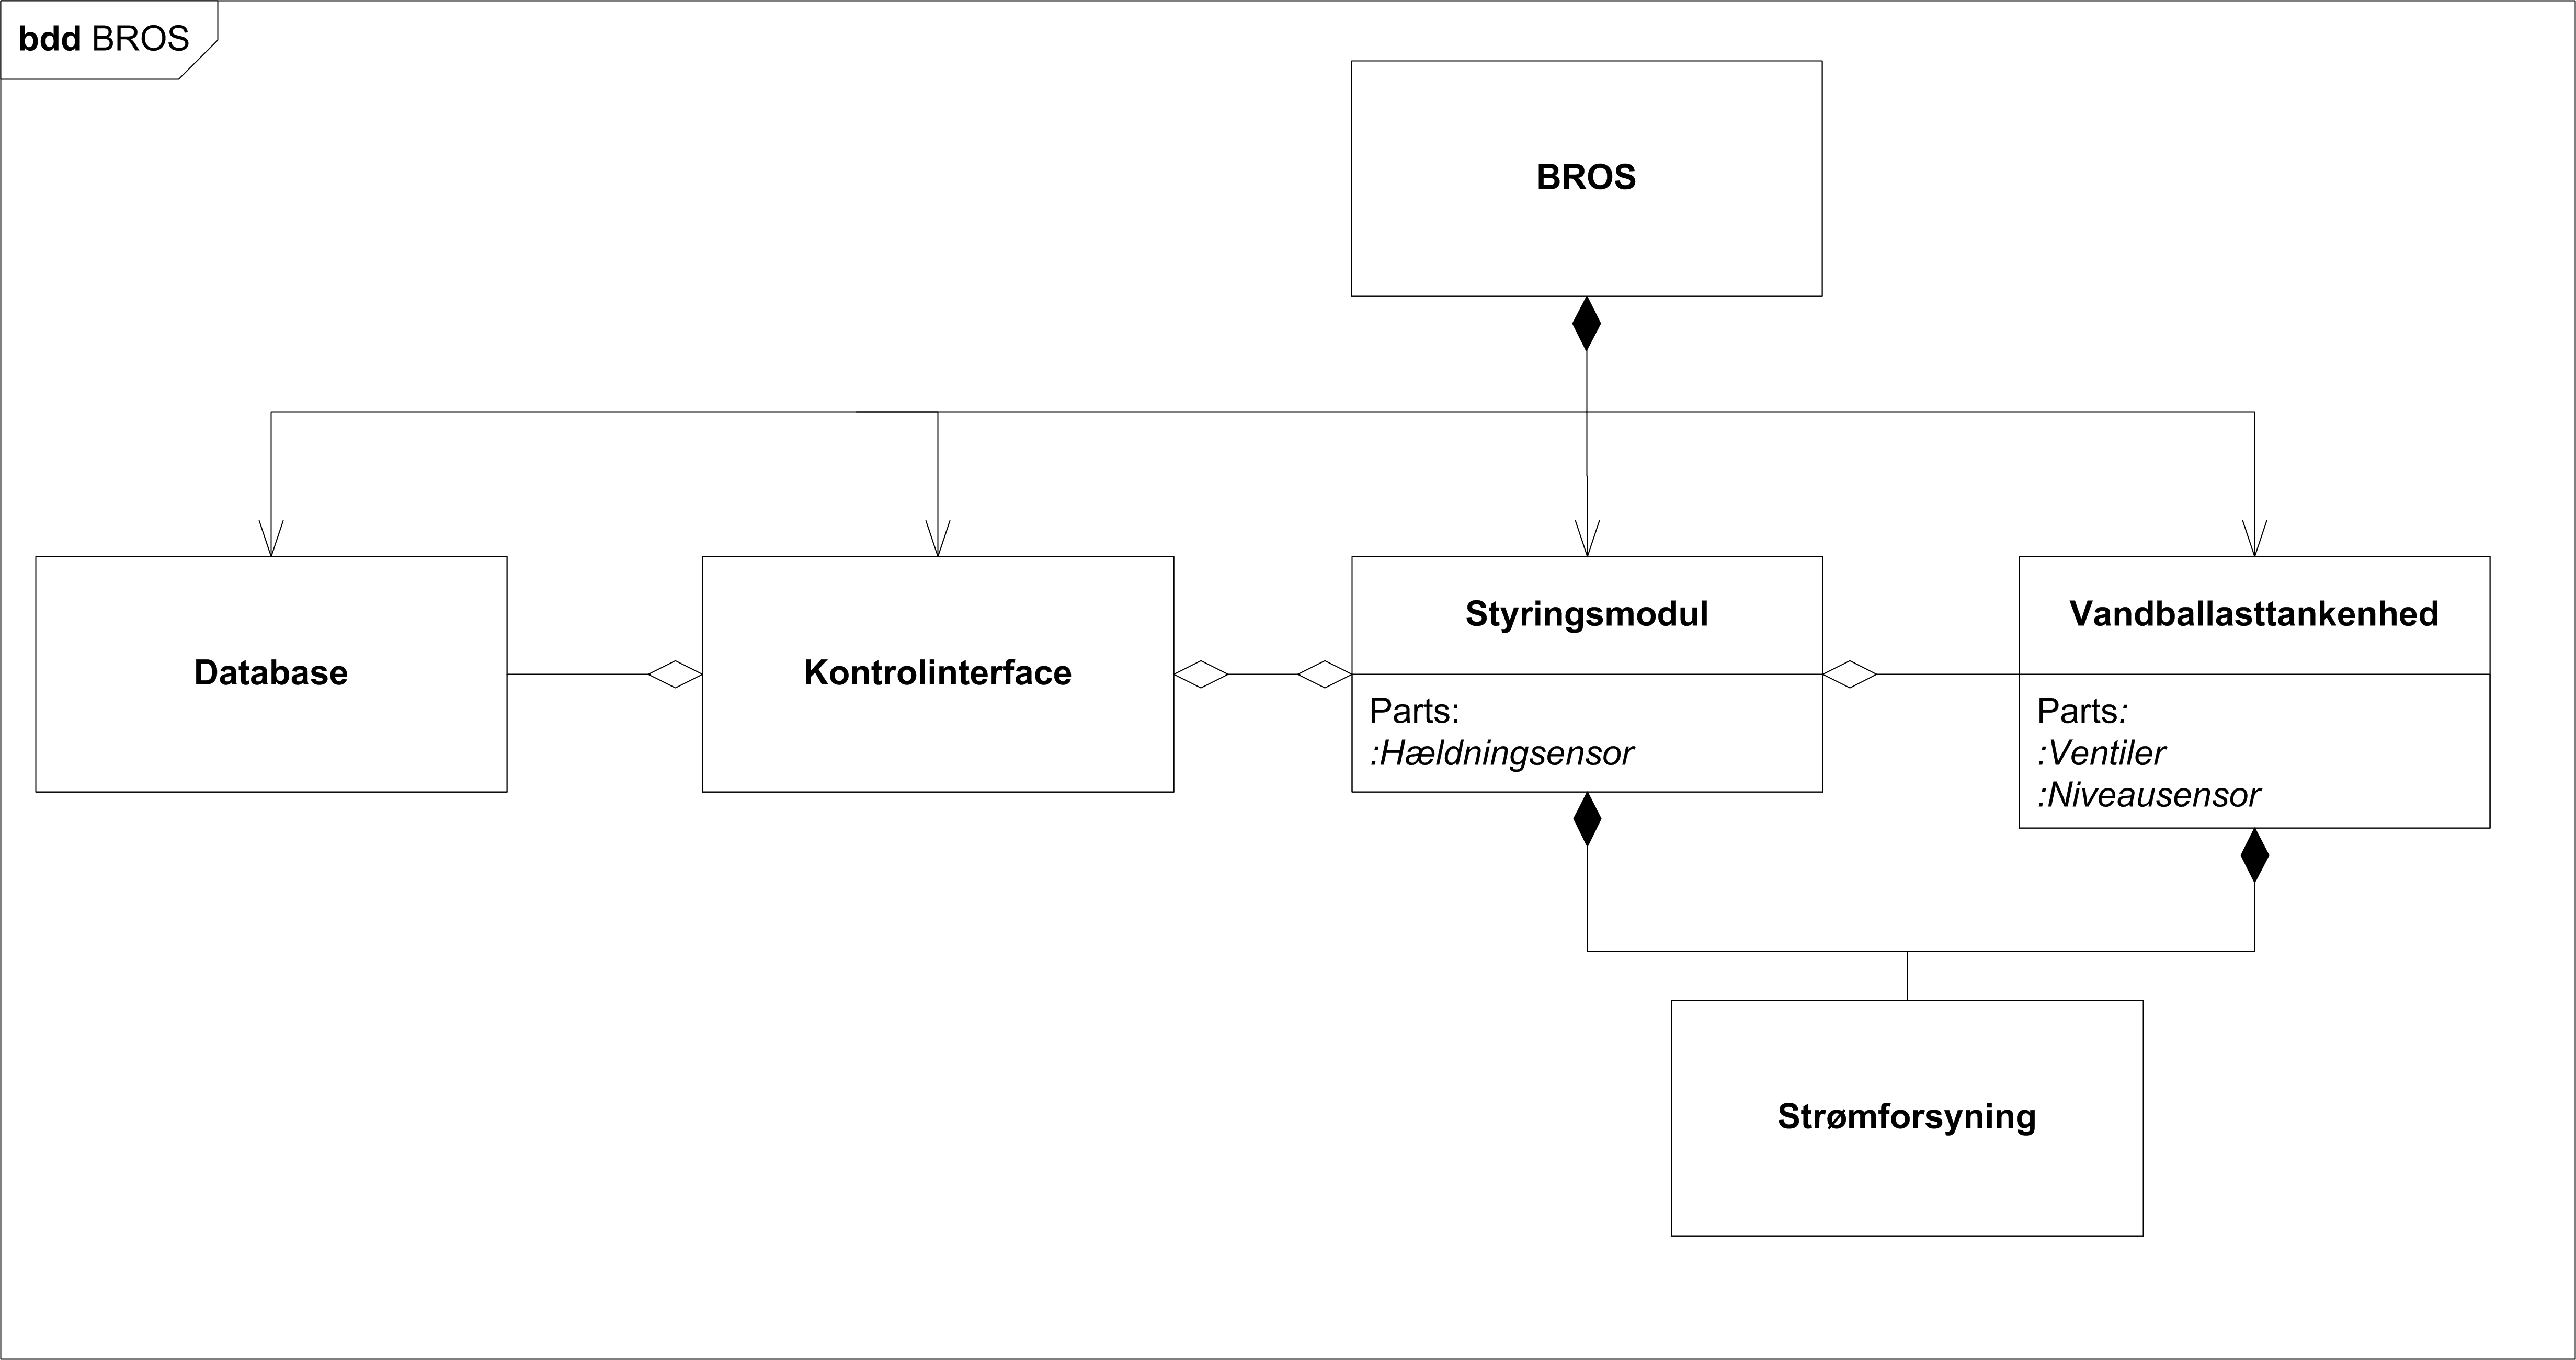
\includegraphics[scale=0.8]{billeder/Systemarkitektur/bdd_bros}
\caption{Blokdefinitionsdiagram for systemet}
\label{fig:bdd_bros}
\end{figure}

Herefter er opgaven to-delt. Kommunikationsvejene skal kortlægges både internt mellem blokkene og for inputs og outputs af systemet. Begge dele gøres i et internt blokdiagram. Det interne blokdiagram for systemet kan ses i figur \ref{fig:idb_bros}. Her angives det også hvor mange gange de enkelte blokke skal optræde i systemet.\\

\fxnote{Indsæt protokoller}
Systemet er nu opdelt i fysiske blokke. For hver blok er der angivet et state machine. Kommunikationsprotokollen imellem blokkene er beskrivet. Designfasen kan påbegynde.

Det endelige produkt skal have strøm fra en strømforsyning \fxnote

\begin{figure}[htbp]
\centering
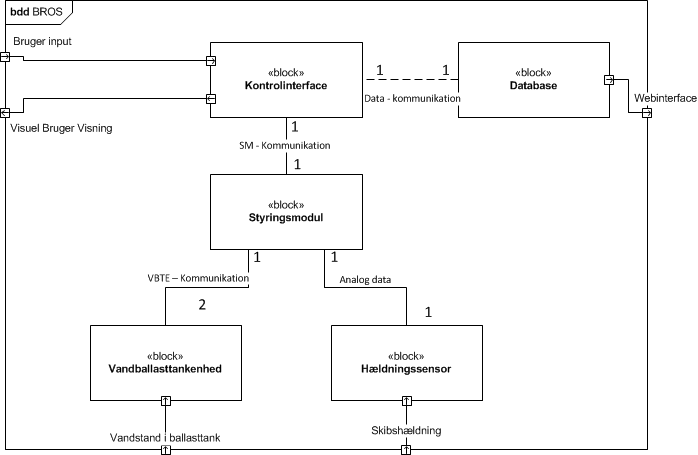
\includegraphics[scale=0.8]{billeder/Systemarkitektur/ibd_bros}
\caption{Internt blokdiagram for systemet}
\label{fig:idb_bros}
\end{figure}

